\documentclass[11pt]{article}

\usepackage{fullpage} 
\usepackage{hyperref}
\usepackage{amsmath}
\usepackage{amssymb}
\usepackage{amsthm}
\usepackage{graphicx}
\usepackage{pgf}
\usepackage{tikz}
\usepackage{longtable}
\usepackage{wasysym}
\usepackage{enumitem}
\usepackage{xcolor}
\usepackage{color, colortbl}
\usepackage{longtable}
\usepackage{datetime}


\usetikzlibrary{arrows,automata}

\usepackage{indentfirst}

\newcommand{\question}[2] {\vspace{0.3in}\noindent{\subsection*{Question #1. #2} \vspace{0.15in}}}

\renewcommand{\part}[1] {{\vspace{0.15in}\noindent\textbf (#1)} \vspace{0.10in}}

\definecolor{dark-blue}{RGB}{23,20,119}
\definecolor{dark-green}{RGB}{2,101,15}
\definecolor{tableheadcolor}{gray}{0.65}
\definecolor{tablerowcolor}{gray}{0.90} 



%  ----------------------------------------------------------------
%                         Start here
% ----------------------------------------------------------------
 
\begin{document}

\title{Assignment \#5} %Replace X with the appropriate number
\author{\Large Gustavo Estrela de Matos\\ %Replace with your name
CSCE 433: Formal Languages and Automata} %If necessary, replace with your course number and title
\date{\today} 

\maketitle

\question{1}{For each of the following languages, construct a PDA to accept $L$. \\
\part{a} $L = \{a^n b^{2n} \mid n \geq 0\}$ \\
\part{b} $L = \{a^ib^jc^k \mid i, j, k \geq 0$ and $i + k = j\}$ \\
\part{c} $L = \{w \mid w$ has twice as many $0$'s as $1$'s$\}$}

\part{a}

The idea for this language PDA is to have a state where the $a$'s are read and for each of them we push $2$ elements in the stack; and a also a state where the $b$'s are read and for each of them an element is poped from the stack. Since we pushed $2$ elements for every $a$ and poped one for every $b$ we can guarantee that when the stack has $z_0$ on the top.

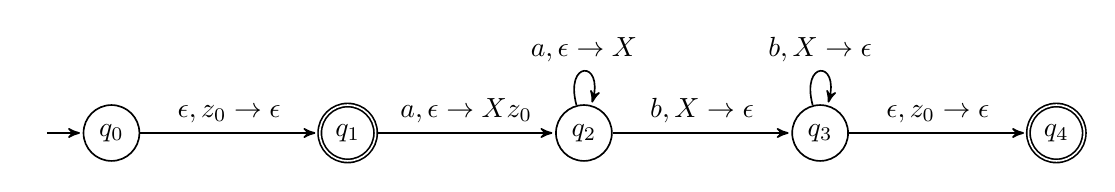
\begin{tikzpicture}[->,>=stealth',shorten >=1pt,auto,node distance=3cm, semithick, initial text={}, align=left]
  
    \tikzstyle{every state}=[fill=white,draw=black,text=black, minimum size=15pt]

    \node[initial,state]    (0)              {$q_0$};
    \node[accepting, state] (1) [right of=0] {$q_1$};
    \node[state]            (2) [right of=1] {$q_2$};
    \node[state]            (3) [right of=2] {$q_3$};
    \node[state, accepting] (4) [right of=3] {$q_4$};
 
    \path (0) edge node {$\epsilon, z_0 \rightarrow \epsilon$}     (1)
          (1) edge node {$a, \epsilon \rightarrow Xz_0$}           (2)
          (2) edge [loop above] node {$a, \epsilon \rightarrow X$} (2)
          (2) edge node {$b, X \rightarrow \epsilon$}              (3)
          (3) edge [loop above] node {$b, X \rightarrow \epsilon$} (3)
          (3) edge node {$\epsilon, z_0 \rightarrow \epsilon$}     (4)
    ;                      
\end{tikzpicture}    

This PDA is deterministic.


\part{b}

Saying that $i + k = j$ is the same as saying that $k = j - i$, therefore we need to calculate $j- i$ while reading $a$s and $b$s. To do that we are going to push an element $X$ for every $a$ and pop them for every $b$ read. Once the stack have $z_0$ on the top we can start pushing $Y$s for every $b$ read. 

The number of $Y$s in the stack after reading all $b$s will be the number of $c$s needed to the input to be in $L$. If after reading all the $b$s we have a $X$ on the top of the stack we know we already know that the string is not in $L$ because having a $X$ on the top means that $j < i$ thus there's no positive $k$ such that $i + k = j$.

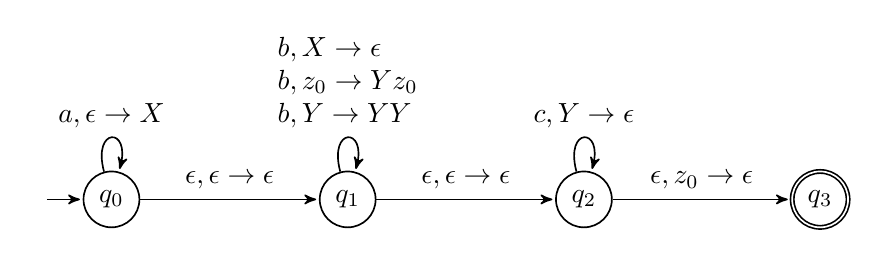
\begin{tikzpicture}[->,>=stealth',shorten >=1pt,auto,node distance=3cm, semithick, initial text={}, align=left]
  
    \tikzstyle{every state}=[fill=white,draw=black,text=black, minimum size=15pt]

    \node[initial,state]    (0)              {$q_0$};
    \node[state]            (1) [right of=0] {$q_1$};
    \node[state]            (2) [right of=1] {$q_2$};
    \node[state, accepting] (3) [right of=2] {$q_3$};
 
    \path (0) edge node {$\epsilon,\epsilon \rightarrow \epsilon$} (1)
          (0) edge [loop above] node {$a,\epsilon \rightarrow X$}  (1)
          (1) edge node {$\epsilon, \epsilon \rightarrow \epsilon$}(2)
          (1) edge [loop above] node {$b, X \rightarrow \epsilon$ \\ 
                                      $b, z_0 \rightarrow Yz_0$   \\
                                      $b, Y \rightarrow YY$}       (1)
          (2) edge [loop above] node {$c, Y \rightarrow \epsilon$} (2)
          (2) edge node {$\epsilon, z_0 \rightarrow \epsilon$}(3)
    ;                      
\end{tikzpicture}    

This PDA is nondeterministic.

\part{c}

To build this DFA we are going to use two symbols:
\begin{itemize}
    \item{$Y$:} the number of $Y$s in the stack will represent the number of $0$s needed for the string to be in $L$;
    \item{$X$:} the number of $X$s in the stack will represent the number of $1$s needed for the string to be in $L$; \\
and the stack will keep the stack with only $z_0$ and either $X$s or $Y$s.
\end{itemize}

Our DFA will have at least two states: one to represent that the string so far read is in $L$ and other state if there are symbols needed to be read for the string to be in $L$. If we are in the second state we need to have a feew rules:
\begin{itemize}
\item{$1, Y \rightarrow YYY$:} if needed $0$s and read a $1$ we need two more $0$.
\item{$0, Y \rightarrow \epsilon$:} if needed $0$s and read a $0$ we need one less $0$.
\item{$1, X \rightarrow \epsilon$:} if needed $1$s and read a $1$ we need one less $1$.
\end{itemize}

But what if we read one more $0$ when needing $1$s? We would need to read one more $1$ and one more $0$. Since we don't want to have mixed $X$s and $Y$s in our stack we will create another state that will represent our need for an amount of $1$s and one more $0$. From this state three things can happen:
\begin{itemize}
    \item{$1, X \rightarrow \epsilon$:} if we read a $1$ we would need one less $1$;
    \item{$\epsilon, z_0 \rightarrow Xz_0$:} if we read all $1$s we needed, then we only need to read one more $0$;
    \item{$0, X \rightarrow XX$:} if we read a $0$ then we only need to read one more $1$ (for the $0$ we read when entering and getting out of this state).
\end{itemize}

Finally, the PDA:


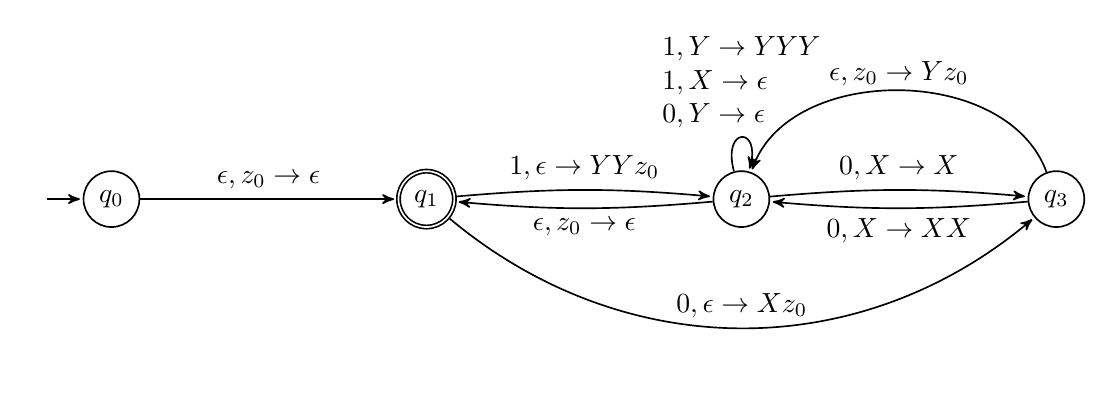
\begin{tikzpicture}[->,>=stealth',shorten >=1pt,auto,node distance=4cm, semithick, initial text={}, align=left]
  
    \tikzstyle{every state}=[fill=white,draw=black,text=black, minimum size=15pt]

    \node[initial,state]    (0)              {$q_0$};
    \node[state, accepting] (1) [right of=0] {$q_1$};
    \node[state]            (2) [right of=1] {$q_2$};
    \node[state]            (3) [right of=2] {$q_3$};
 
    \path (0) edge node {$\epsilon, z_0 \rightarrow \epsilon$}      (1)
          (1) edge [bend left = 5] node {$1, \epsilon \rightarrow YYz_0$} (2)
          (1) edge [bend right = 40] node {$0, \epsilon \rightarrow Xz_0$} (3)
          (2) edge [bend left = 5] node {$\epsilon, z_0 \rightarrow \epsilon$} (1)
          (2) edge [loop above] node {$1, Y \rightarrow YYY$ \\
                                      $1, X \rightarrow \epsilon$ \\
                                      $0, Y \rightarrow \epsilon$} (2)
          (2) edge [bend left = 5] node {$0, X \rightarrow X$} (3)
          (3) edge [bend left = 5] node {$0, X \rightarrow XX$} (2)
          (3) edge [bend right = 70] node [yshift = 5mm] {$\epsilon, z_0 \rightarrow Yz_0$} (2)
    ;                      
\end{tikzpicture}    


\question{2}{
    Consider the following context-free grammar $G = (\{S, S_1, S_2, X\}, \{a, b\}, R, S)$, where $R$ consists of the following rules:
\begin{center}
\begin{tabular}{l c l}
    $S$   & $\rightarrow$ & $S_1 | S_2 $ \\
    $S_1$ & $\rightarrow$ & $aS_1a | bS_1b | \epsilon $ \\
    $S_2$ & $\rightarrow$ & $XXS_2 | X$ \\
    $X$   & $\rightarrow$ & $a | b$ \\
\end{tabular}
\end{center}
\part{a} Give a succinct English description of $L(G)$. \\
\part{b} Is the context-free grammar $G$ ambiguous? Justify your answer. \\
\part{c} Give a one-state PDA $M$ that accepts $L(G)$. \\
\part{d} For your PDA $M$, show an accepting computation path for the string $abba$.\\
\part{e} For your PDA $M$, show an accepting computation path for the string $bbb$.
}

\part{a}
This CFL represents strings of $a$s and $b$s that are palindromo or with odd length.

\part{b} 
Considering the CFLs with starting symbol $S_1$ and $S_2$ we can see that both are not ambiguous. Since $S$ is the union of these two CFLs and they don't have any string in common (because one has only strings of odd length and other only with even length) we can say that $S$ is also not ambiguous.

\part{c}
\begin{center}
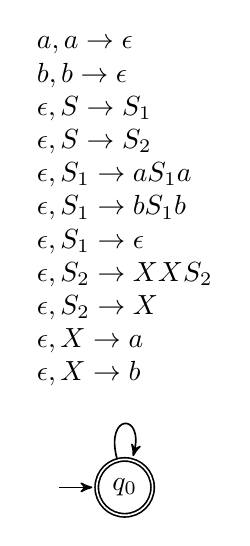
\begin{tikzpicture}[->,>=stealth',shorten >=1pt,auto,node distance=4cm, semithick, initial text={}, align=left]
  
    \tikzstyle{every state}=[fill=white,draw=black,text=black, minimum size=15pt]

    \node[initial, accepting, state] (0) {$q_0$};
 
    \path (0) edge [loop above] node {$a, a \rightarrow \epsilon$ \\
                         $b, b \rightarrow \epsilon$ \\
                         $\epsilon, S \rightarrow S_1$ \\
                         $\epsilon, S \rightarrow S_2$ \\
                         $\epsilon, S_1 \rightarrow aS_1a$ \\
                         $\epsilon, S_1 \rightarrow bS_1b$ \\
                         $\epsilon, S_1 \rightarrow \epsilon$ \\
                         $\epsilon, S_2 \rightarrow XXS_2$ \\
                         $\epsilon, S_2 \rightarrow X$ \\
                         $\epsilon, X \rightarrow a$ \\
                         $\epsilon, X \rightarrow b$ \\
    }      (0)
    ;                      
\end{tikzpicture}    
\end{center}

\part{d}
$(q, abba, S) \vdash (q, abba, S_1) \vdash (q, abba, aS_1a) \vdash (q, bba, S_1a) \vdash (q, bba, bS_1ba) \vdash (q, ba, S_1ba) \vdash (q, ba, ba) \vdash (q, a, a) \vdash (q, \epsilon, \epsilon)$.

\part{e}
$(q, bbb, S) \vdash (q, bbb, S_2) \vdash (q, bbb, XXS_2) \vdash (q, bbb, bXS_2) \vdash (q, bb, XS_2) \vdash (q, bb, bS_2) 
\vdash (q, b, S_2)
\vdash (q, b, X)
\vdash (q, b, b)
\vdash (q, \epsilon, \epsilon)
$


\question{3}{In each case, use the pumping lemma to show that the given language is not a CFL.\\
\part{a} $L = \{a^ib^jc^k \mid k = max (i, j)\}$ \\
\part{b} $L = \{w \in \{a, b, c\}^* \mid \eta_a(w) < \eta_b(w) < eta_c(w)\}$. The number of $a$'s, $b$'s, and $c$'s in the string $w$ are represented by $\eta_a(w)$, $\eta_b(w)$ and $\eta_c(w)\}$ respectively.
}

\part{a}

Assume that $L$ is a CFL.  Let $p$ be the pumping constant.  Choose the string $s$ to be $a^pb^pc^p$.  Since the $|s| \geq p$, then $s$ can be broken up into 5 pieces $u,v,x,y$ and $z$, such that:
\begin{itemize}
	\item $|vy| \geq 1$,
	\item $|vxy| \leq p$, and
	\item for all $i \geq 0$, $uv^ixy^iz \in L$.
\end{itemize} 

\noindent 
We must consider the following ways of partitioning the string $s$ into $u,v,x,y$, and $z$. We list partitions based on the contents of $v$ and $y$ since they affect the pumped string $s'$.

\begin{longtable}{|c|c|c|c|p{2in}|p{2.75in}|} \hline
%\multicolumn{6}{|c|}{Let $s = a^pb^pc^p$.} \\ \hline 
\rowcolor{tableheadcolor} 
   & $v$ & $y$ & $i$ & $s'=uv^ixw^iy$ & Why is $s' \notin L$?\\ \hline 
\rowcolor{tablerowcolor}
\multicolumn{6}{|c|}{$vx$ contains a single distinct symbol} \\ \hline 
1. & $a^l$ & $a^m$ & 2 & $a^{p+l+m)}b^pc^p$ & Number of $a$'s is greater than the number of $c$'s. \\ [0.3cm]

2. & $b^l$ & $b^m$ & 2 & $a^pb^{p+l+m}c^p$ & Number of $b$'s is greater than the number of $c$'s. \\ [0.3cm]
	
3. & $c^l$ & $c^m$ & 0 & $a^pb^pc^{p-(l+m)}$ & Number of $c$'s is less than $p = max (p, p)$. \\ [0.3cm]

\hline
\rowcolor{tablerowcolor}
\multicolumn{6}{|c|}{$v$ and $y$ contain two different distinct symbols} \\ \hline 

4. & $a^l$ & $b^m$ & 2 & $a^{p+l}b^{p+m}c^p$ & Since $l$ and $m$ are greater than zero (otherwise, case 1 or 2)we have that $p$ can't be $max(p + l, p + m)$. \\ [0.3cm]	

5. & $b^l$ & $c^m$ & 0 & $a^pb^{p-l}c^{p-m}$ & Since $m$ is greater than zero (otherwise, case 2) we have that $p - m$ can't be $max (p, p - l)$. \\ [0.3cm] 

\hline 

\rowcolor{tablerowcolor}
\multicolumn{6}{|c|}{$v$ or $x$ contain 2 distinct symbols} \\ \hline 

6. & $a^l$ & $a^mb^n$  & 0 & $a^{p - (l + m)}b^{p-n}c^p$ & Since $l$, $m$ and $n$ are greater than zero (othewise, case 1, 2, 4) we have that the number of $c$'s is greater than $max (p - (l + m), p - n)$\\ [0.7cm]

7. & $a^l b^m$ & $b^n$  & 0 & $a^{p-l}b^{p-(m + n)}c^p$ &  Since $l$, $m$ and $n$ are greater than zero (othewise, case 1, 2, 4) we have that the number of $c$'s is greater than $max (p - l, p - (n + m))$. \\ [0.7cm]	

\hline 

8. & $b^l$ & $b^mc^n$  & 0 & $a^pb^{p-(l + m)}c^{p-n}$ & Since $n$ is greater than zero (otherwise, case 2) we have that the number of $c$'s is less than $max (p, p - (l + m))$  \\ [0.7cm] 

\hline 

9. & $b^l c^m$ & $c^n$  & 2 & $a^{p} b^{p-l} c^{p - (m + n)}$ & Since $n$ and $m$ are greater than zero (otherwise, case 2 or 5) we have that the number of $c$'s is less than $max (p, p - l)$ \\ 

\hline 
\end{longtable}

The above cases show that no matter how we partition the string $s$ into $u,v,x, y$, and $z$, the resulting pumped string $s'$ will not be in the language $L$.  Thus, our assumption that $L$ is context-free is false. 

\part{b}

Assume that $L$ is a CFL.  Let $p$ be the pumping constant.  Choose the string $s$ to be $a^pb^{p+1}c^{p+2}$.  Since the $|s| \geq p$, then $s$ can be broken up into 5 pieces $u,v,x,y$ and $z$, such that:
\begin{itemize}
	\item $|vy| \geq 1$,
	\item $|vxy| \leq p$, and
	\item for all $i \geq 0$, $uv^ixy^iz \in L$.
\end{itemize} 

\noindent 
We must consider the following ways of partitioning the string $s$ into $u,v,x,y$, and $z$. We list partitions based on the contents of $v$ and $y$ since they affect the pumped string $s'$.

\begin{longtable}{|c|c|c|c|p{2in}|p{2.75in}|} \hline
%\multicolumn{6}{|c|}{Let $s = a^pb^pc^p$.} \\ \hline 
\rowcolor{tableheadcolor} 
   & $v$ & $y$ & $i$ & $s'=uv^ixw^iy$ & Why is $s' \notin L$?\\ \hline 
\rowcolor{tablerowcolor}
\multicolumn{6}{|c|}{$vx$ contains a single distinct symbol} \\ \hline 
1. & $a^l$ & $a^m$ & 2 & $a^{p+l+m}b^{p+1}c^{p+2}$ & Since $l + m > 0$, the number of $a$'s is greater  or equal than the number of $b$'s. \\ [0.3cm]

2. & $b^l$ & $b^m$ & 2 & $a^pb^{p+l+m}c^p$ & Since $l + m > 0$, the number of $b$'s is greater or equal than the number of $c$'s. \\ [0.3cm]
	
3. & $c^l$ & $c^m$ & 0 & $a^pb^{p + 1}c^{p + 2 -(l+m)}$ & Since $l + m >0$, the number of $c$'s is less or equal than the number of $b$'s. \\ [0.3cm]

\hline
\rowcolor{tablerowcolor}
\multicolumn{6}{|c|}{$v$ and $y$ contain two different distinct symbols} \\ \hline 

4. & $a^l$ & $b^m$ & 2 & $a^{p+l}b^{p+1+m}c^{p+2}$ & Since $m$ is greater than zero (otherwise, case 1) we have that the number of $b$'s is greater or equal to the number of $c$'s. \\ [0.3cm]	

5. & $b^l$ & $c^m$ & 0 & $a^pb^{p - l + 1}c^{p - m + 2}$ & Since $l$ is greater than zero (otherwise, case 3) we have that the number of $b$'s is less or equal than the number of $a$'s. \\ [0.3cm] 

\hline 

\rowcolor{tablerowcolor}
\multicolumn{6}{|c|}{$v$ or $x$ contain 2 distinct symbols} \\ \hline 

6. & $a^l$ & $a^mb^n$  & 2 & $a^{p  + l + m}b^{p + n + 1}c^{p + 2}$ & Since $n$ is greater than zero (othewise, case 1) we have that the number of $b$'s is greater or equal to the number of $c$'s \\ [0.7cm]

7. & $a^l b^m$ & $b^n$  & 2 & $a^{p + l}b^{p + m + n + 1}c^{p + 2}$ &  Since $m$ and $n$ are greater than zero (othewise, case 1, 4) we have that the number of $b$'s is greater or equal than the number of $c$'s. \\ [0.7cm]	

\hline 

8. & $b^l$ & $b^mc^n$  & 0 & $a^pb^{p - (l + m) + 1}c^{p + 2 - n}$ & Since $l$ and $m$ are greater than zero (otherwise, case 3 or 5) we have that the number of $b$'s is less than the number of $a$'s  \\ [0.7cm] 

\hline 

9. & $b^l c^m$ & $c^n$  & 0 & $a^{p} b^{p - l + 1} c^{p - (m + n) + 2}$ & Since $n$ and $m$ are greater than zero (otherwise, case 3 or 5) we have that the number of $c$'s is less than the number of $b$'s. \\ 

\hline 
\end{longtable}

The above cases show that no matter how we partition the string $s$ into $u,v,x, y$, and $z$, the resulting pumped string $s'$ will not be in the language $L$.  Thus, our assumption that $L$ is context-free is false. 




\question{4}{For each of the following languages, determine whether it is context-free or not, and a proof for your answer. \\
\part{a} $L = \{xayb \mid x, y \in \{a,b\}^*$ and $|x| = |y|\}$ \\
\part{b} $L = \{xyx \mid x, y \in \{a, b\}^*$ and $|x| \geq 1\}$ \\
\part{c} $L = \{(ab^n)^n \mid n \geq 0\}$
}

\end{document}
